\section{Chasing the Fundamental Harmonic}
%heating up and chasing the ....
As a second experiment to measure the change in frequency and so velocity
of second sound with changing temperature. 

The cryogenic environment is slowly heated up using the already calibrated 
resistor from section \ref{sec:cal} for the temperature measurement.

\subsection{Theory}
The second sound requires the two fluid model to propagate, but the 
ratio of superfluid to normal fluid changes over temperature.
at $T = T_B$ there is no more superfluid,
specifically the velocity depends on the ratio according to:
$$c^2 = \underbrace{\frac{\rho_s}{\rho_n}}_{ = 0 \text{ at } T>T_B} \cdot \frac{T S^2}{C_v}$$
from Equation \ref{equ:c2rsrnts2cv} (page \pageref{equ:c2rsrnts2cv}).

\subsection{Method}
The frequency generator is set to the first node.
The pipe to the vacuum pump is closed and the pressure from the boiling helium starts to increase.


The liquid helium is not in equilibrium with the vapour and heats up
with the net heat flow from the environment.
It is not possible to use measurements of pressure
to get the temperature, so the Allen Bradley resistor and 
the calibration is used.

During heating measurements of the resistance and frequency of the
first harmonic are taken.
The frequency is located using the `live' method similar to finding the frequency for
the $n= \{3,4,\ldots\}$ harmonics. Excepts at the frequency is constantly dropping
the operator predicted the frequency and then without tuning the signal generator a 
maxima is observed on the phase signal amplifier, this works well when the 
rate of change of frequency was small, but above $\approx2.0$K the rate of 
change of frequency was larger and the uncertainty that are approximated  
the the operator are very large.

The top AB resistor in Figure \ref{fig:pseuphysicsview} is used for measuring the resistance.

\subsection{Results}

The Frequency and calculated temperatures are plotted in Figure \ref{fig:fundementalchasing}.
It shows that the velocity depends on the temperature as the frequency of the first harmonic.

At high temperatures, towards $T_k$, the frequency of the first harmonic drops to $0$.

The fitting used is a cubic only because it seems to fit the data well.
There is an apparent peak of the frequency at $1.675\pm 0.5$, this could be from
a beneficial radio of superfluid and normalfluid components.
\begin{figure*}[htbp]
\centering
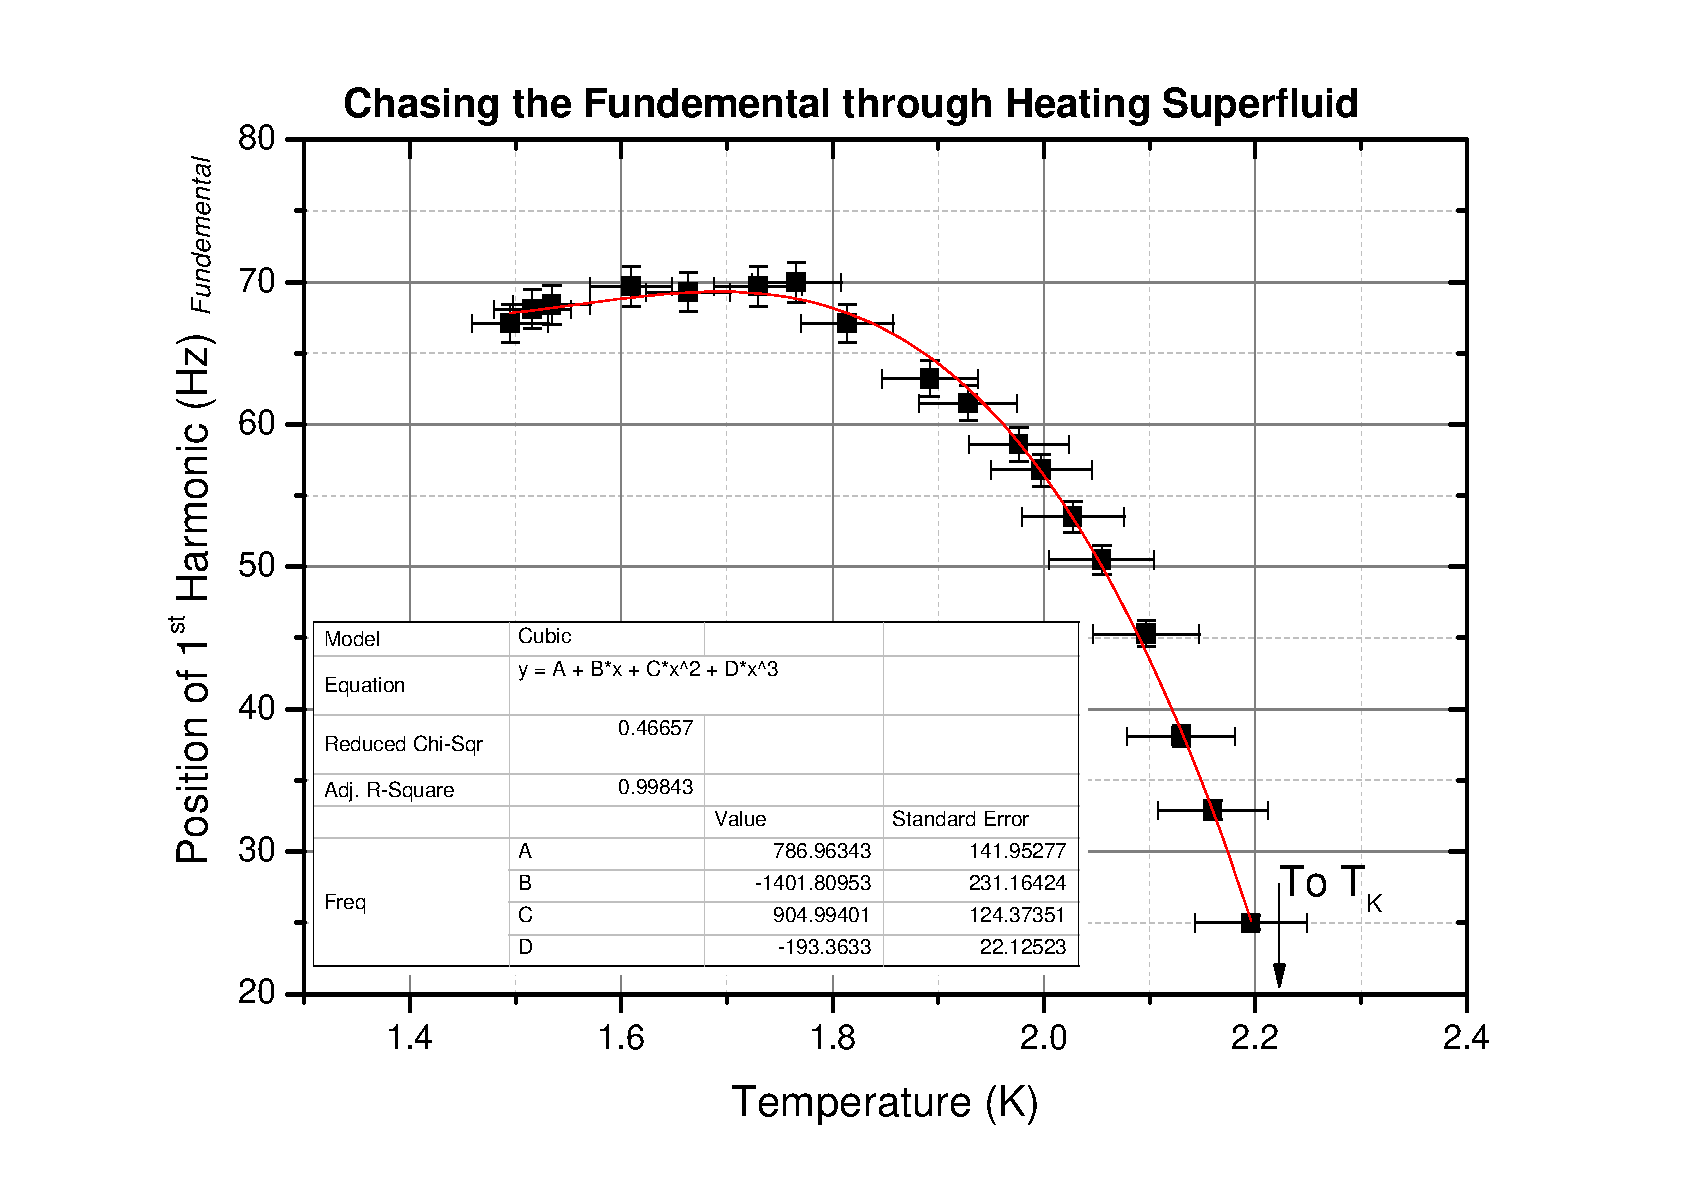
\includegraphics[width = 0.8\textwidth]{pics/fundementalchasing.pdf}
\caption{Plot of the fundamental frequency against temperature calculated from
the resistance of the Allen-Bradley resistor during cooling \label{fig:fundementalchasing}}
\end{figure*}


